\section{Benchmarks}
\label{sec:benchmarks}

This Section lists the programs on which the compiler was evaluated, and the results of the experiements performed. Due to a lack of a capable standard library (see Section \ref{sec:javalib}), the number of eligible real-world, CPU-intensive Java benchmarks was limited. This, coupled with the lack of well-maintained Java front-end for LLVM meant that we instead opted to write our own example programs on which to test the quality of the compiled code. These programs are not `benchmarks' as such, as they do not test a compiler as thoroughly as the SPEC benchmark suite does, for example. They do, however, give a general insight as to the performance of our compiler's resulting code on everyday user applications.

Each program was first compiled to a Dalvik executable file via the standard procedure. Each was written in Java with the Eclipse IDE, then exported as a .jar file. The \verb|dx| tool, as bundled with the Android SDK, was then used to convert the Java archive to the Dalvik executable format. At this point our compiler was run to translated this file to LLVM intermediate representation. This file was treated as our `base' file. In order to examine the effect LLVM's optimization passes had on code performance, the bytecode was further optimized using the LLVM \verb|opt| tool. In particular, three additional bytecode files were produced, each run with a base optimization setting of \verb|-mem2reg -std-compile-opts -std-link-opts|. The \verb|mem2reg| pass, as described earlier, promotes stack values and memory to registers, and is one of the vital optmization passes the compiler relies upon. The \verb|std-compile-opts| pass activates a standard list of compile-time optimization passes. The standard list of link-time optimizations is likewise given by the \verb|std-link-opts| flag.

The three main flags run on the bytecode file were the \verb|-O1|, \verb|-O2|, and \verb|-O3| optimization settings. These roughly correspond to the respective optimization flags offered by the GCC compiler.

Source code for all benchmarks is listed in the Appendix.

\subsection*{Array}

The `array' benchmark declares an array of 50,000,000 integers, assigns them values and then prints them back out. As arrays and looping are so ubiquitous in programming, it is important to test their performance in order to gain insight into how the compiler performs on common applications. The printing of the array values is important, as although the print function call might become a performance bottleneck in this situation, without it neither the Dalvik or optimized LLVM bytecodes ever actually assign the array values.

\begin{figure}[h!]
    \centering
    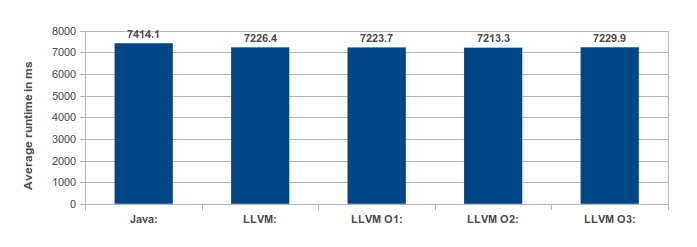
\includegraphics[width=1.0\textwidth]{images/res_array.png}
    \caption{Execution times of `array' benchmark}
    \label{fig:res_array}
\end{figure}



\subsection*{Factors}

The `factors' benchmark attempts to find the factors of a given $N$ through a brute-force approach. This program is again designed to test loop performance, with additional computation inside each loop iteration. In this case, the program was tasked with finding the factors of the long value $1,000,000,014,000,000,049$.

\begin{figure}[h!]
    \centering
    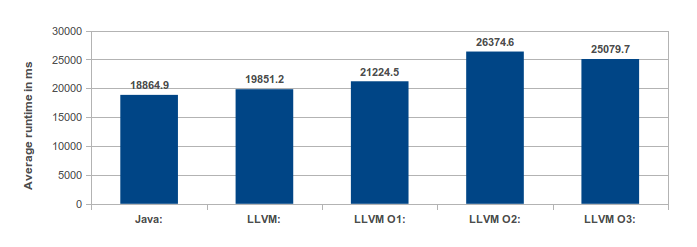
\includegraphics[width=1.0\textwidth]{images/res_factors.png}
    \caption{Execution times of `factors' benchmark}
    \label{fig:res_factors}
\end{figure}

The translated LLVM bytecode performed well here, with its average runtime of 19,851 milliseconds closely resembling that of the Java's 18,864 milliseconds. Those LLVM versions that were passed through the LLVM optimizer did not fare so well, with the \verb|-O3| version


\subsection*{Fibonacci}

The 'fibonacci' benchmark, as its name suggests, computes the fibonacci numbers up to and including a given $N$. This program is function-call- and recursion-intensive, and is designed to test the compiler's ability to handle efficient function calls. The following results were taken from running the program with $N = 40$.

\begin{figure}[h!]
    \centering
    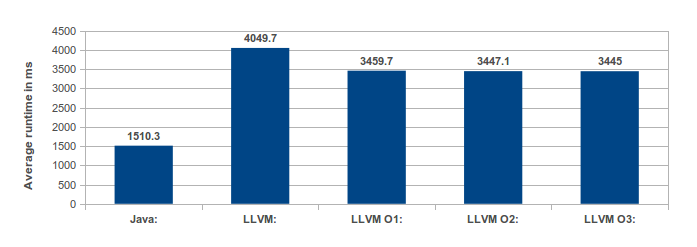
\includegraphics[width=1.0\textwidth]{images/res_fibonacci.png}
    \caption{Execution times of `fibonacci' benchmark}
    \label{fig:res_fibonacci}
\end{figure}

The results in Figure \ref{fig:res_fibonacci} indicate that the function call performance of LLVM cannot perform at the level the JVM offers. The Java bytecode version of the program reported an average runtime of 1,510 milliseconds, and the highest-performing LLVM version - that optmizied at \verb|-O3| level - achieved a runtime of 3,445 milliseconds.


\subsection*{Primes}

The `primes' benchmark finds and prints the all prime numbers up to a given $N$, again through a brute-force approach. It aims to give a good indication of the performance of loops with additional computation, such as division and modulus arithmetic. The results shown were taken from the program computing the prime numbers up to $N = 100,000$.

\begin{figure}[h!]
    \centering
    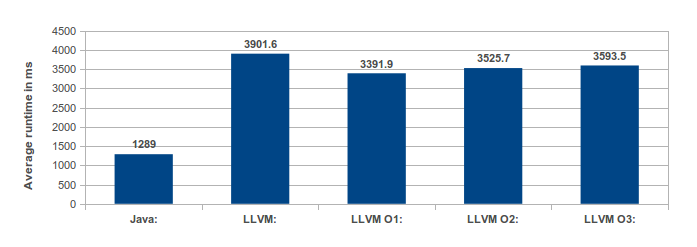
\includegraphics[width=1.0\textwidth]{images/res_primes.png}
    \caption{Execution times of `primes' benchmark}
    \label{fig:res_primes}
\end{figure}

Looking at the results in Figure \ref{fig:res_primes} we can see the performance gap between the Java and LLVM bytecode versions of the benchmark. On average the LLVM programs took over three times as long to compute and display the prime numbers, with the \verb|-O1| optimized version proving the best of the LLVM representations.

It must be noted, however, that our compiler is at a disadvantage in this case especially. Due to Dalvik's type inference of registers (see Section \ref{sec:typeinf}), our compiler uses 64-bit integers as a solution. Regardless of whether a value is of \verb|int| or \verb|long| type, the resulting LLVM code will use a 64-bit integer. With a large amount of integer computation, as in the `primes' benchmark, this is likely to create a disparity between the performance of both systems.

To create a fairer comparison between the Java and LLVM versions of the program, we additionally evaluated the benchmark using \verb|long| computation. The results in Figure \ref{fig:res_primes_long} display the average runtimes of the `primes' benchmark using computation of \verb|long| values. The use of 64 bit integers in the LLVM bytecode is evidently detrimental to performance, as the disparity between runtimes as shown in Figure \ref{fig:res_primes} has largely been mitigated. The optimized versions of the LLVM bytecode perform nearly on par with the Java version in this case. This is a huge oversight in the design of the compiler, and the redesign in future work to use 32-bit integers where appropriate will be vital to the optimal performance of the system.

\begin{figure}[h!]
    \centering
    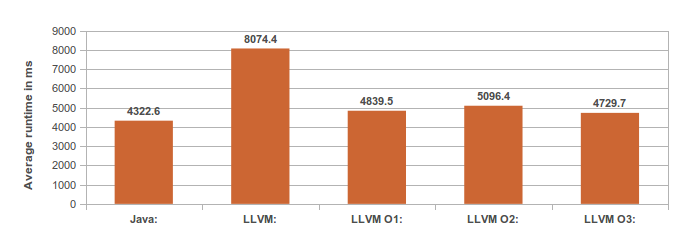
\includegraphics[width=1.0\textwidth]{images/res_primes_long.png}
    \caption{Execution times of long-computation `primes' benchmark}
    \label{fig:res_primes_long}
\end{figure}
